\section{Introduction}
Work presented in previous chapters highlighted the much improved \textit{ab initio} decoy quality achievable by restraining the conformational search space with residue-residue contact information. Furthermore, the data also highlighted that this improvement extends AMPLE's tractability of achieving structure solution for more challenging targets. However, the data also indicated that AMPLE's current protocol is not tailored towards decoy sets with overall much higher accuracy. Decoy sets with correctly predicted folds (average \gls{tmscore} $>0.5$ per 1,000 decoys) did not generate any or many ensemble search models leading to \gls{mr} structure solution. It also became apparent that certain decoy sets contained few high-quality decoys that were lost in the process of clustering, since non of the top-10 SPICKER clusters contained that fold.

Beyond the limitations observed in AMPLE, \textit{ab initio} decoy similarity in exceptional cases approaches a near-identical fold (RMSD $<1.5$\AA) to the crystallised one. Although challenging by current means to identify these decoys, it is of great interest since these decoys might be sufficient by themselves as \gls{mr} search models. Contact information, which was used to restrain the folding protocol, might provide enough information to drive such filtering. Indeed, \textcite{De_Oliveira2017-gj} found that long-range residue-residue contact pair satisfaction correlates well with decoy quality. Additionally, \textcite{Adhikari2018-lj} use long-range contact satisfaction routinely in CONFOLD2 to exclude the worst decoys amongst the set predicted ones.

Thus, this chapter focuses on exploring alternative strategies of decoy selection in AMPLE, and if contact information can be used beyond the distance-restraint application in \textit{ab initio} protein structure prediction.

\section{Materials \& Methods}
\subsection{Target selection}
The dataset for this study consisted of 113 ROSETTA decoy sets generated throughout the works outlined in previous chapters. The 113 decoy sets covered all targets in the ORIGINAL (\cref{table:appendix_dataset_original}), PREDICTORS (\cref{table:appendix_dataset_predictors}) and TRANSMEMBRANE (\cref{table:appendix_dataset_transmembrane}) datasets. Top-$L$ ($>5$ residues sequence separation) CCMPRED \cite{Seemayer2014-zp}, PCONSC2 \cite{Skwark2014-qp}, METAPSICOV STAGE 1 \cite{Jones2015-vq} and MEMBRAIN \cite{Yang2013-bf} contact pairs were used in combination with the \textit{FADE} energy function to restrain the \textit{ab initio} structure prediction process.

\subsection{Computation of range-specific satisfaction scores}
The satisfaction of short- ($>6$ residues sequence separation), medium- ($>12$ residues sequence separation) and long-range contact pairs ($>23$ residues sequence separation; see \cref{sec:methods_longrange_satisfaction}) were computed for each decoy in each set. Hereby, the contact pairs of the original set of contact pairs used to restrain the \textit{ab initio} structure prediction protocol were extracted, matched against the contact pairs extracted from individual decoys and the contact pair range-specific satisfaction score evaluated. 

\subsection{Decoy subselection} \label{sec:ample_decoys_decoy_selection}
Each set of decoys was ranked in descending order by their long-range contact pair satisfaction scores and the $n$ decoys with the lowest scores removed from each set. The number of decoys to remove $n$ was selected using a number of different strategies:

\begin{description}[style=multiline,leftmargin=3cm]
    \item[\textit{NONE}] leave the original set unchanged
    \item[\textit{LINEAR}] remove the worst 500 decoys
    \item[\textit{CUTOFF}] remove all decoys with a score of $<0.287$ 
    \item[\textit{SCALED}] remove all decoys with a scaled score of $<0.5$, where the scaled score is score divided by set average
\end{description}

The fixed definition in the \textit{CUTOFF} strategy was determined by \textcite{De_Oliveira2017-gj}. The scaled score used by the \textit{SCALED} strategy was computed by dividing each decoy's long-range contact pair satisfaction by the set's average.

Furthermore, an \textit{INDIVIDUAL} subselection strategy was employed, which differed substantially from the others. The top-5 decoys by long-range contact satisfaction were selected and subjected to treatment outside of AMPLE. The per-decoy treatments were the following:

\begin{description}[style=multiline,leftmargin=3cm]
    \item[default] leave the decoy unchanged
    \item[bfactor] remove all residues with a CONCOORD \cite{De_Groot1997-gb} B-factor of less than 30\AA\textsuperscript{2}
    \item[domain] remove all residues with $kde<\frac{1}{2}max_{kde}$, where $kde$ corresponds to the \gls{kde} and $max_{kde}$ to the maximum \gls{kde} obtained by applying the algorithm described by \textcite{Sadowski2013-zu} to the top-5$L$ contact map
    \item[dssp] remove all residues that were assigned secondary structure by DSSP \cite{Frishman1995-si} not in \{$H, B, E, G, I$\}
    \item[residue] remove all residues that do not form a consecutive fragment of at least 3 residues in the top-$L$ contact map
    \item[variance] remove all residues with cluster variance computed by THESEUS \cite{Theobald2006-qj} of more than 5\AA\ (cluster variance determined from \textit{NONE} strategy)
\end{description}

\subsection{Molecular Replacement} \label{subsec:ample_decoys_methods_mr}
To evaluate the benefits of such subselection to \gls{mr} in AMPLE, a subset of 35 decoy sets (spanning 35 unique targets) were processed as described above and subjected to AMPLE v1.2.0 and CCP4 v7.0.28. Default options were chosen with few exceptions: decoys in all 10 clusters were used, subcluster radii thresholds were set to 1 and 3\AA, and side-chain treatments were set to \texttt{polyala} only. This change in protocol was shown to be advantageous in most cases by \textcite{Thomas2017-qu}, and thus trialled in this context. 

To allow comparability of these results to previous AMPLE runs, an additional condition was added, namely \textit{NONE\_classic}. The decoy set from the \textit{NONE} strategy was hereby subjected to the AMPLE protocol with default settings except \texttt{-num\_clusters}, which was set to sample the three largest clusters.

All individual decoys created under \textit{INDIVIDUAL} strategy were subjected as poly-Alanine decoys to MRBUMP \cite{Keegan2018-kn} with identical settings to those used in AMPLE. 

Each \gls{mr} run was assessed using the criteria defined in \cref{sec:methods_mr_success}.

\section{Results}
This chapter focuses on identifying further uses of predicted residue-residue contact pairs in unconventional \gls{mr}. In particular, the exclusion of \textit{ab initio} decoys by their contact satisfaction scores is under investigation. A total of 113 decoy datasets were used to identify potential means of identifying the best or worst decoys. Furthermore, three strategies were trialled alongside two standards to test the viability of excluding the worst decoys in ensemble search model preparation in AMPLE.

\subsection{Contact pair satisfaction correlates with decoy quality}
\textcite{Kosciolek2014-bt} previously identified a correlation between the TM-score of a decoy and its fraction of satisfied contact pairs. Albeit the striking positive correlations (short-range:$\rho=0.50$; medium-range:$\rho=0.57$; long-range:$\rho=0.87$) for top-1 decoys, the study by \textcite{Kosciolek2014-bt} was limited to 10 representative targets with a maximum chain length of 158 residues. Furthermore, FRAGFOLD \cite{Jones2001-mc} was used for \textit{ab initio} protein structure prediction, a method with inferior performance to ROSETTA \cite{Rohl2004-dj} when using the decoys in unconventional \gls{mr} (see \cref{chap:alternate_abinitio_protocols}). Thus, the more diverse set of decoys generated in this study might be more representative in determining a correlation between decoy TM-scores and contact pair satisfaction.

A correlation analysis with 35 ROSETTA decoy sets representing 35 globular and transmembrane targets shows a positive linear correlations between a decoy's TM-score and short-, medium- and long-range contact satisfaction (\cref{table:ample_decoys_tmscore_consat}). Furthermore, separating the correlation analysis of all targets by fold classification reveals that all-\textalpha, mixed \textalpha-\textbeta\ and transmembrane protein targets show the strongest positive correlations for long-range contact satisfaction (\cref{table:ample_decoys_tmscore_consat}). All-\textbeta\ and mixed \textalpha-\textbeta\ decoy sets show the strongest correlations for short- and medium-range contact satisfaction, whereby the former shows a stronger positive correlation between the decoy's TM-score and its medium-range contact satisfaction than its long-range contact satisfaction (medium-range:$\rho=0.54$; long-range:$\rho=0.50$) (\cref{table:ample_decoys_tmscore_consat}). Notably, the decoys of transmembrane protein targets show no correlation between TM-score and short-range contact satisfaction ($\rho=0.08$; \cref{table:ample_decoys_tmscore_consat}).

\begin{table}[H]
  \centering
  \caption[Correlation analysis between decoy TM-score and contact satisfaction]{Pearson's \gls{cc} analysis between a ROSETTA decoy's TM-score and short-, medium- and long-range contact satisfaction. Probability values for all \textrho coefficients is $<0.01$.}
  \label{table:ample_decoys_tmscore_consat}
  \begin{tabularx}{\textwidth}{X X X X}
      \hline
      \multirow{2}{*}{\textbf{Target class}} & \multicolumn{3}{c}{\textbf{Pearson's \gls{cc}}} \\ \cline{2-4}
      & Short-range   & Medium-range  & Long-range \\
      \hline
      all                               & 0.11          & 0.18          & 0.64 \\
      all-\textalpha                    & 0.30          & 0.44          & 0.69 \\
      all-\textbeta                     & 0.40          & 0.54          & 0.50 \\
      mixed \textalpha-\textbeta        & 0.42          & 0.55          & 0.69 \\
      transmembrane                     & 0.08          & 0.48          & 0.70 \\
      \hline
  \end{tabularx}
\end{table}

Following on from the correlation analysis, a linear regression model was fitted to individual subsets of the data used for the correlation analysis to see if a decoy's TM-score could be predicted from its contact satisfaction score. However, weak coefficients of determination indicate that only some cases show models with reasonably good fits to the data (\cref{fig:ample_decoys_smlrcstmfold}). Nevertheless, all models further support the positive linear correlations between a decoy's TM-score and its range-dependent contact satisfaction. Interestingly, the strongest and best fits of the linear regression model to its corresponding data is for long-range contact pairs, where the linear regression models are also near identical between the different fold categories (\cref{fig:ample_decoys_smlrcstmfold}).

\begin{figure}[H]
	\centering
	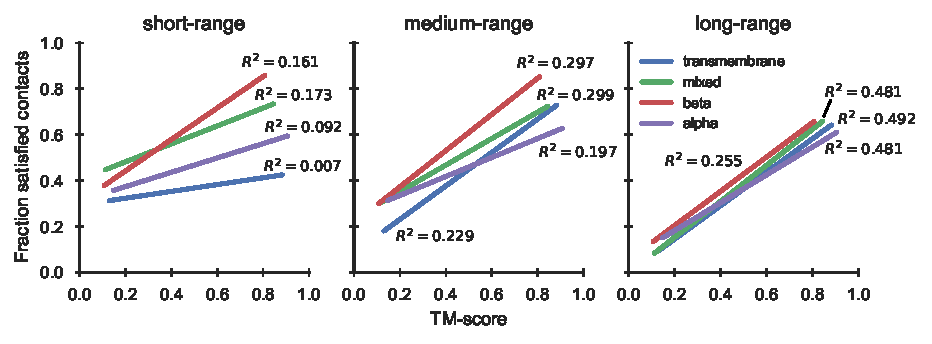
\includegraphics[width=\textwidth]{ample_decoys_smlrcstmfold.pdf}
        \caption[Linear regression model between decoy TM-score and contact satisfaction]{Linear regression model fitted to decoy TM-scores and corresponding fractions of satisfied, range-dependent contacts. Targets were further separated by fold classification. Ceofficients of determination ($R^2$-values) added alongside each regression model.}
	\label{fig:ample_decoys_smlrcstmfold}
\end{figure}

An analysis of the correlation between the TM-score and long-range contact satisfaction of individual decoy sets further highlights the potential to subselect decoy sets by their long-range contact satisfaction. Thirty decoy sets show statistically significant positive correlations between decoy TM-scores and their long-range contact satisfaction ($\rho$-values in range of 0.09 to 0.97 with p-value $<0.01$). A singleton ROSETTA decoy set, derived for the Glycolipid transfer protein with \gls{pdb} ID 2eum and restrained with METAPSICOV STAGE 1 contact data, shows a weak negative correlation ($\rho=-0.10$, $p<0.01$). The remaining four decoy sets, derived for targets with \gls{pdb} IDs 1chd, 1gm4, 2x6u and 3ouf and restrained with METAPSICOV STAGE 1 contact data except for 2x6u (PCONSC2), show no statistically significant correlation between the TM-score and long-range contact satisfaction of the decoy sets. 

A further subdivide of the previously presented data by metapredictor highlights that no predictor outperforms the others. Decoy sets from all metapredictors result in decoy sets with stronger and weaker correlations. Similarly, target chain length and fold do not show overall stronger or weaker correlations. 

So far, all analyses focused on entire sets of decoys (1,000 decoys per set); however, it is often desirable to know if we could better estimate the accuracy of the best decoy by some measure. \textcite{Kosciolek2014-bt} demonstrated strong positive correlations for short-, medium- and long-range contact satisfaction with a decoy's corresponding TM-score. In this work, these findings are confirmed albeit the strength of the correlation for long-range contact satisfaction is much weaker than observed previously (short-range: no correlation; medium-range:$\rho=0.52$; long-range:$\rho=0.69$) (\cref{fig:ample_decoys_smlrcstmtop1}). The weak positive correlation for short-range contact satisfaction is statistically non-significant, and thus cannot be validated. 

\begin{figure}[H]
	\centering
        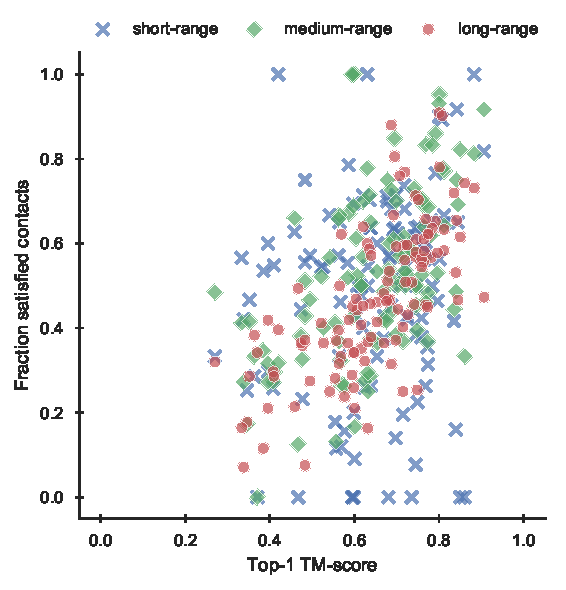
\includegraphics[width=0.7\textwidth]{ample_decoys_smlrcstmtop1.pdf}
        \caption[Top-1 decoy TM-score and contact satisfaction analysis]{Analysis of the relationship between TM-score and contact satisfaction for the top-1 decoy (as ranked by TM-score) in each decoy set.}
	\label{fig:ample_decoys_smlrcstmtop1}
\end{figure}




% - How many decoys do we exclude for the different selection criteria?
% - How does the correlation affect the selection of decoys?
% - How do the exclusion conditions affect the quality measures of our decoy sets?
% - How does the selection impact AMPLE ensemble search model generation?
% - How does decoy exclusion impact MR?

\subsection{Long-range contact satisfaction metric to filter decoy sets}
In the previous section, the data highlighted that decoy quality correlates positively with contact satisfaction. In particular, a strong positive correlation between long-range contact satisfaction and decoy quality could be established for almost all decoy sets in this study. A key ambition in this work is to determine, if this correlation could be used to include or exclude decoys prior to submission to the AMPLE processing pipeline to enrich the quality and number of ensemble search models trialled in \gls{mr}. 

The difference in mean TM-score of each decoy set before and after applying a subselection strategy (see \cref{sec:ample_decoys_decoy_selection}) is shown in \cref{fig:ample_decoys_deltatmsub}. Estimating a decoy's quality by short-range contact satisfaction results in marginal mean TM-score changes of decoy sets ($\Delta_{CUTOFF}=-0.003$; $\Delta_{LINEAR}=0.008$; $\Delta_{CUTOFF}=0.001$). In comparison, medium- ($\Delta_{CUTOFF}=0.005$; $\Delta_{LINEAR}=0.015$; $\Delta_{CUTOFF}=0.002$) and long-range ($\Delta_{CUTOFF}=0.025$; $\Delta_{LINEAR}=0.032$; $\Delta_{CUTOFF}=0.005$) contact satisfaction are better estimates to improve the mean TM-score values of each decoy set. Notably, per-decoy long-range contact satisfaction provides the best estimate for identifying and excluding the least accurate decoys independent of the subselection strategy. 

\begin{figure}[H]
	\centering
	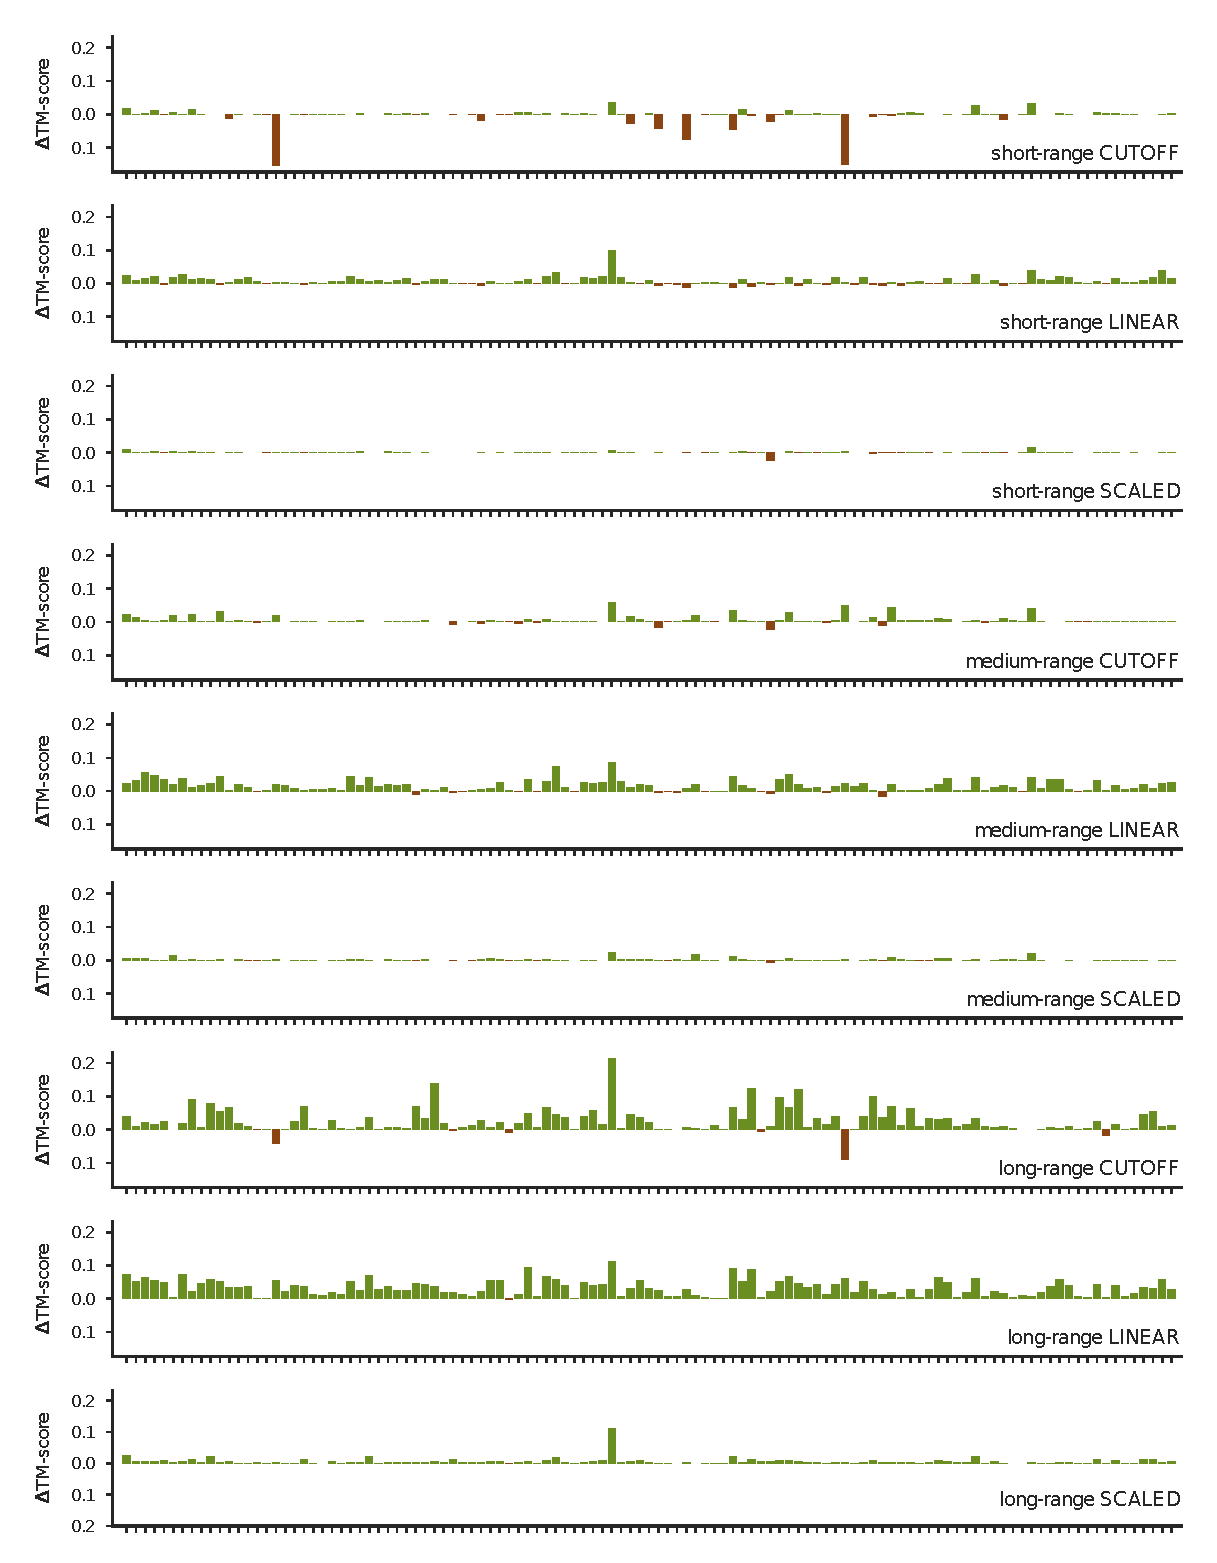
\includegraphics[width=\textwidth]{ample_decoys_deltatmsub.pdf}
        \caption[TM-score comparison pre- and post-decoy subselection]{Differences in mean TM-score  for decoy sets pre- and post-decoy subselection. Each subselection strategy is stated in each subplot along with the contact range used to establish decoy inclusion in the final set.}
	\label{fig:ample_decoys_deltatmsub}
\end{figure}

A comparison of \textDelta TM-scores between subselection strategies shows that the \textit{LINEAR} strategy results in the largest improvements across all contact range categories. Nevertheless, such great changes are expected compared to other strategies since the \textit{LINEAR} strategy removes on average the most decoys from each set (\textit{CUTOFF}=280; \textit{LINEAR}=500; \textit{SCALED}=66). However, the sample-dependent strategies (\textit{CUTOFF} and \textit{SCALED}) may remove a much greater number of decoys from a set if the corresponding satisfaction scores fall below a certain threshold.

In certain cases, some subselection strategies greatly changed the overall size and quality of the starting decoy set. The METAPSICOV STAGE 1 decoy set of the ankyrin sequence (\gls{pdb} ID: 2qyj) shows overall quality improvements from 0.006 (short-range \textit{SCALED}; $n_{models}=958$) to 0.213 (long-range \textit{CUTOFF}; $n_{models}=218$). The CCMPRED decoy set of sensory rhodopsin II sequence (\gls{pdb} ID: 1gu8) shows overall changes from -0.155 (short-range \textit{CUTOFF}; $n_{models}=2$) to 0.06 (long-range \textit{LINEAR}; $n_{models}=500$).

Overall, the optimal strategy to select or exclude decoys from a starting set of structures appears to be long-range contact satisfaction given the improved similarity metric of the set compared to the reference crystal structure. 


\subsection{AMPLE's cluster-and-truncate approach with filtered decoy sets}
The original dataset was limited to a sub-sample of 35 decoy sets spanning 35 unique targets (21 globular and 14 transmembrane targets) for \gls{mr} trials. The contact prediction algorithms generating the restraints for the \textit{ab initio} structure predictions were PCONSC2 (globular targets) and CCMPRED (transmembrane targets). Each decoy set was subjected to the AMPLE pipeline with certain decoys removed according to one of five subselection strategies.

The initial step in the AMPLE pipeline is the clustering of decoys. A comparison of SPICKER clusters between the \textit{NONE} default strategy and the \textit{CUTOFF}, \textit{LINEAR} and \textit{SCALED} subselection strategies highlights an important difference. Larger clusters --- those ranked higher --- show higher similarity between a subselection strategy and the default (\cref{fig:ample_decoys_jaccluster}). The top SPICKER cluster shows high similarities between the \textit{NONE} strategy and all other subselection ones, whereby it has to be noted that the \textit{LINEAR} strategy contains only 50\% of the starting decoys and thus can at most show a Jaccard index of 0.5. With increasing cluster index, the overall similarity degrades and most of the decoys in cluster 10 are non-identical between each subselection strategy and the default. Furthermore, a similar analysis to compare the overall quality of each cluster compared to the target structure revealed less difference between the default and each subselection strategy for higher-order SPICKER clusters (\cref{fig:ample_decoys_tmcluster}). With decreasing SPICKER cluster index, the difference in median TM-scores starts to alternate without any particular pattern. Thus, pre-selecting decoys prior to AMPLE's cluster-and-truncate approach most certainly preserves the top cluster for the \textit{CUTOFF} and \textit{SCALED} subselection strategies, whereby lower clusters show more deviation from the default.

\begin{figure}[H]
    \centering
    \begin{subfigure}[b]{\textwidth}
        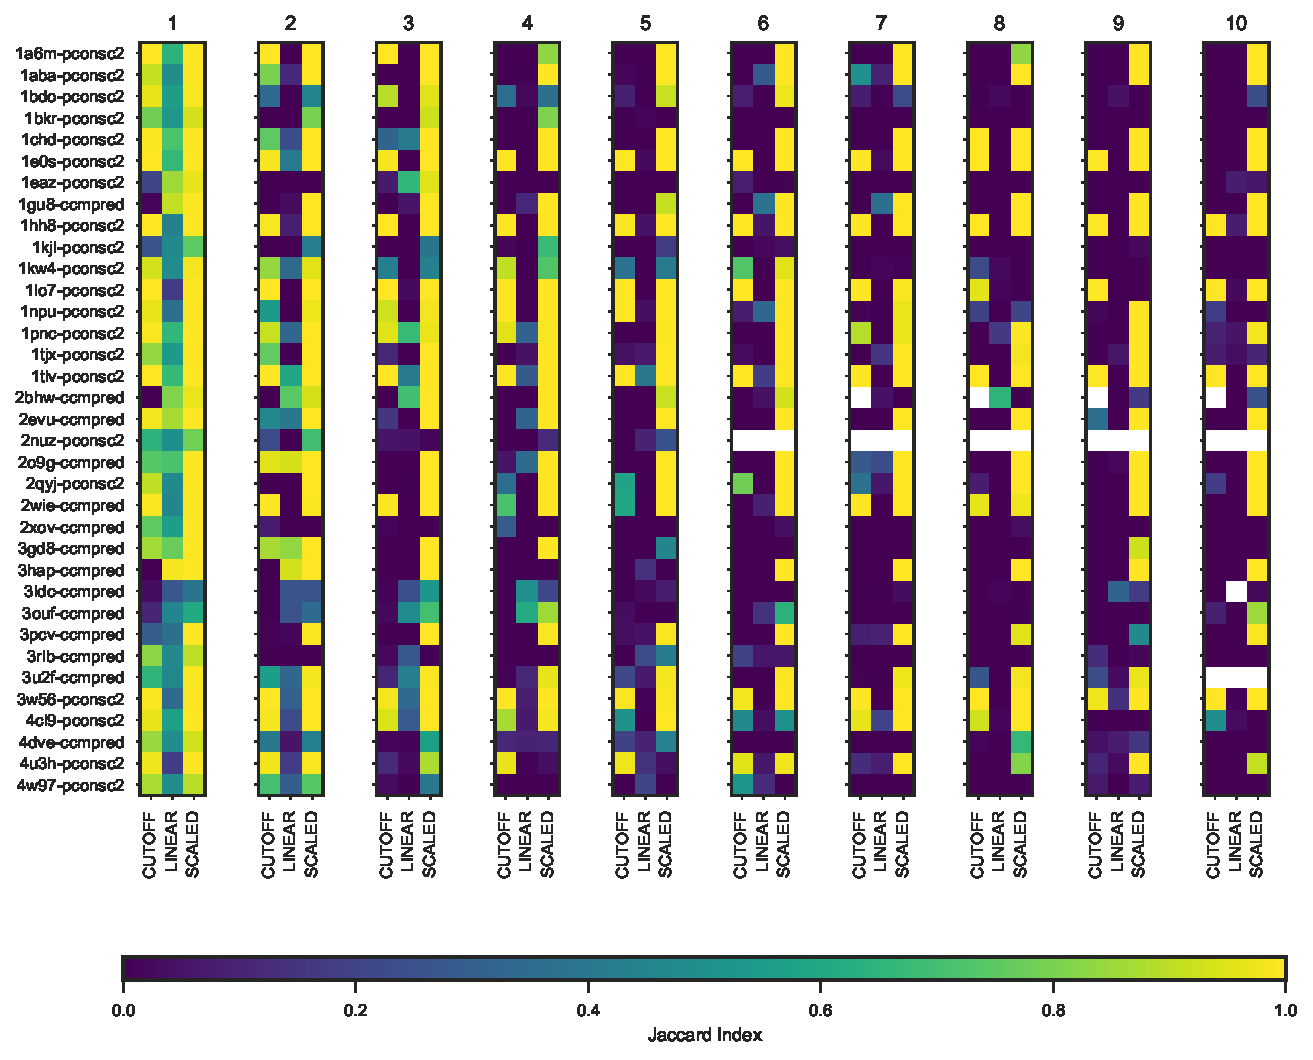
\includegraphics[width=\textwidth]{ample_decoys_jaccluster.pdf}
        \caption{}
        \label{fig:ample_decoys_jaccluster}
    \end{subfigure}
\end{figure}

\begin{figure}[H]\ContinuedFloat
    \begin{subfigure}[b]{\textwidth}
        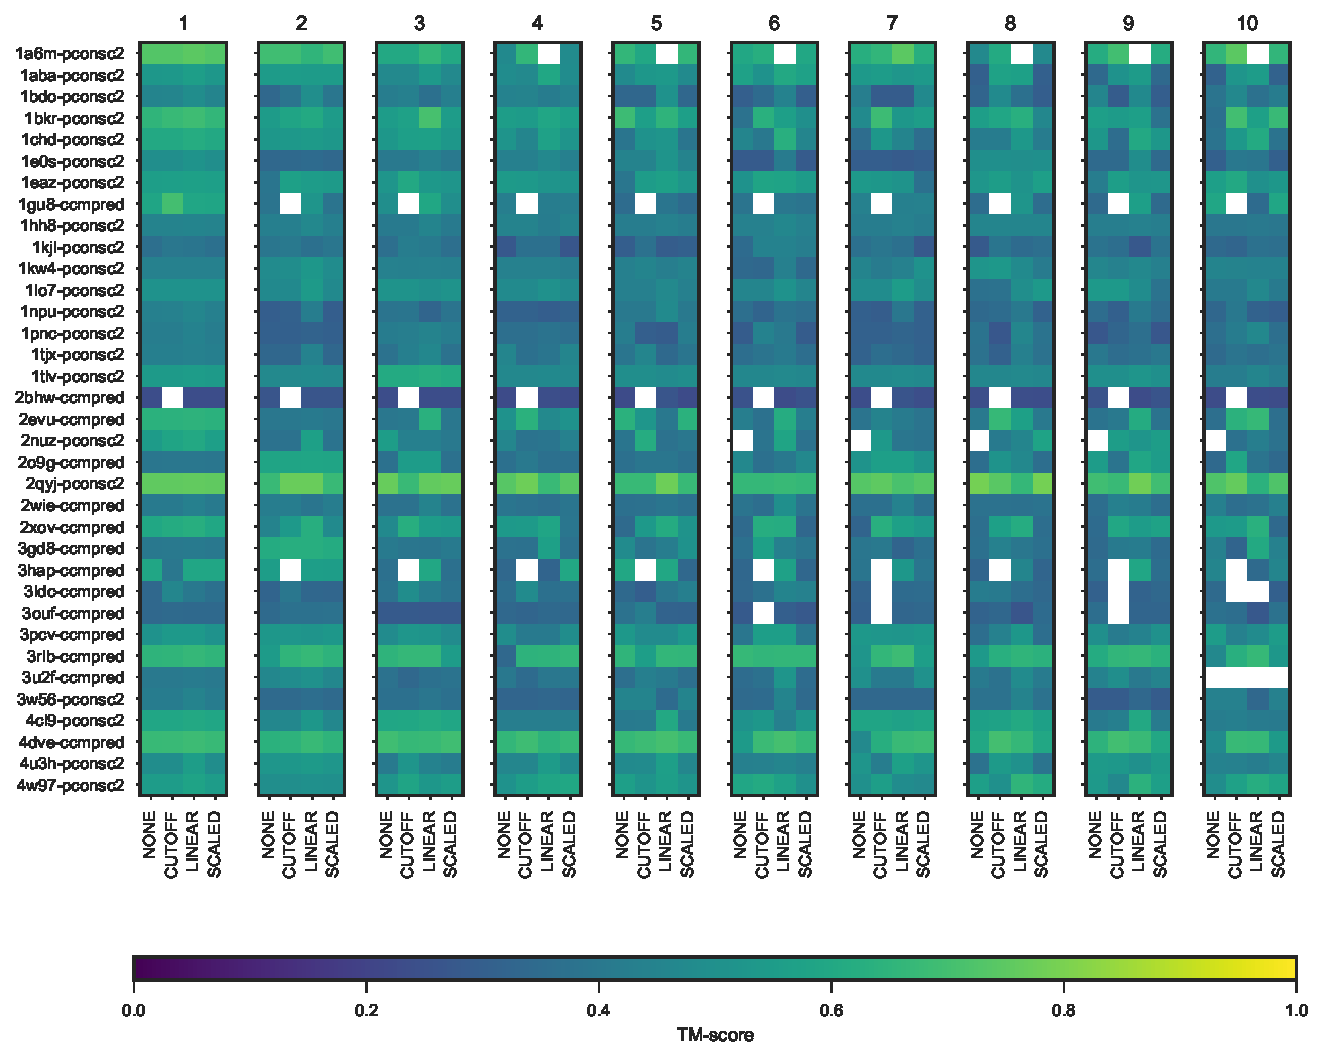
\includegraphics[width=\textwidth]{ample_decoys_tmcluster.pdf}
        \caption{}
        \label{fig:ample_decoys_tmcluster}
    \end{subfigure}
    \caption[Effect of decoy subselection on SPICKER clusters]{Effect of decoy subselection on SPICKER clusters. Effect illustrated by (a) the Jaccard Index and (b) median TM-score difference. Values were calculated for clusters resulting from the full starting set of decoys and the \textit{CUTOFF}, \textit{LINEAR} and \textit{SCALED} subselection strategies.}
\end{figure}

The mean of the inter-decoy variance computed by THESEUS --- used in AMPLE to guide truncation --- is reduced in lower clusters compared to the \textit{NONE} default strategy (\cref{fig:ample_decoys_vardeltacluster}). The clusters of decoys based on the galectin-3 domain (\gls{pdb} ID: 1kjl) sequence show overall the highest reduction in mean inter-decoy variance up to -15\AA compared to the default strategy. Similarly, clusters 4 and 8 of the K\textsuperscript{+}-channel protein domain (\gls{pdb} ID: 3ouf) show reductions in mean inter-decoy variance of up to -20\AA. In general and also true for the aforementioned examples, clusters starting from \textit{CUTOFF}-subselected decoys show mean inter-decoy variance reductions, followed by \textit{LINEAR} and then \textit{SCALED}-subselected decoys sets.

\begin{figure}[H]
    \centering
    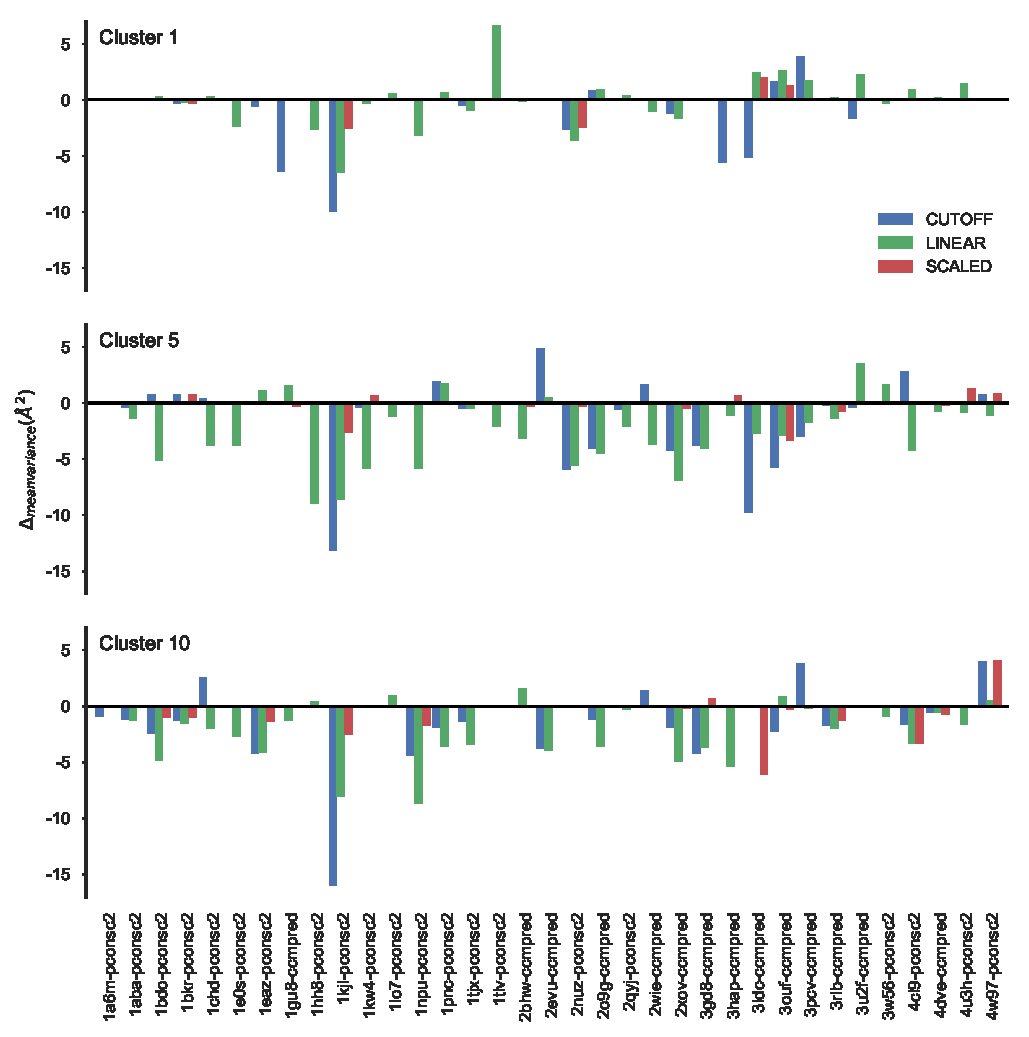
\includegraphics[width=\textwidth]{ample_decoys_vardeltacluster.pdf}
    \caption[Effect of decoy subselection on THESEUS variance]{Effect of decoy subselection on mean inter-decoy THESEUS variance. Difference in mean variance calculated between the default and the three decoy subselection strategies \textit{CUTOFF}, \textit{LINEAR} and \textit{SCALED}. Data for clusters 1, 5 and 10 shown as examples.}
    \label{fig:ample_decoys_vardeltacluster}
\end{figure}

A comparisons of intermediate stages in AMPLE pipeline resulting from differently subselected decoy sets is very difficult. Each strategy results in different starting sets, which result in different clusters. Since AMPLE's objective truncation procedure is based on the inter-decoy variance, it might be greatly affected by differing clusters. Nevertheless, structure solution is more likely when AMPLE generates more ensemble search models because a greater number of search models relates to greater inter-cluster decoy similarity and trialling a greater number should provide a higher chance of success. A count of generated AMPLE ensemble search models reveals that the \textit{SCALED} strategy generates the most search models ($n=7,611$), which is roughly 300 more than the default \textit{NONE} strategy ($n=7,340$). The \textit{CUTOFF} subselection strategy generates the least ensemble search models ($n=7,237$), whilst the \textit{LINEAR} strategy's count ($n=7,401$) is very similar to the \textit{NONE} one.

Further inspection of the number of AMPLE-generated ensemble search models by target reveal near identical numbers between the \textit{NONE}, \textit{LINEAR} and \textit{SCALED} strategies (\cref{fig:ample_decoys_mrsuccesstarget}). In fact, only few outliers for each of those methods distinguish them from the others. The \textit{CUTOFF} strategy shows greater deviation from the other three, especially for certain targets with differences up to approximately 200 ensemble search models (\cref{fig:ample_decoys_mrsuccesstarget}). If we compare all these strategies to the previous default processing in AMPLE (\textit{NONE\_classic}; further details in \cref{subsec:ample_decoys_methods_mr}), we can see that the number of search models is greatly reduced (\cref{fig:ample_decoys_mrsuccesstarget}). A comparison of the previous default (\textit{NONE\_classic}) with the new one (\textit{NONE}) shows on average 144 fewer ensemble search models, whilst sampling a larger range of folds through all 10 clusters.

\subsection{Decoy subselection extends AMPLE's performance}
The final step in this study is the assessment of AMPLE-generate ensemble search models in \gls{mr}. In particular, the comparison of different decoy subselection strategies is of great interest since it might allow us to extend AMPLE's performance beyond that described in previous chapters.

A comparison of the total number of targets solved by each subselection strategy shows that the \textit{CUTOFF}-subselected decoys lead to most structure solutions (14 out of 35) (\cref{fig:ample_decoys_mrsuccesstarget}). Although slightly less successful, the \textit{LINEAR} and \textit{SCALED} subselection strategies lead to approximately 6\% more solved targets than the current AMPLE default \textit{NONE} strategy. The \textit{LINEAR} and \textit{SCALED} strategies are on par with AMPLE's previous default, the \textit{NONE\_classic} strategy (\cref{fig:ample_decoys_mrsuccesstarget}), and thus subselection is needed to achieve the previous performance.

\begin{figure}[H]
    \centering
    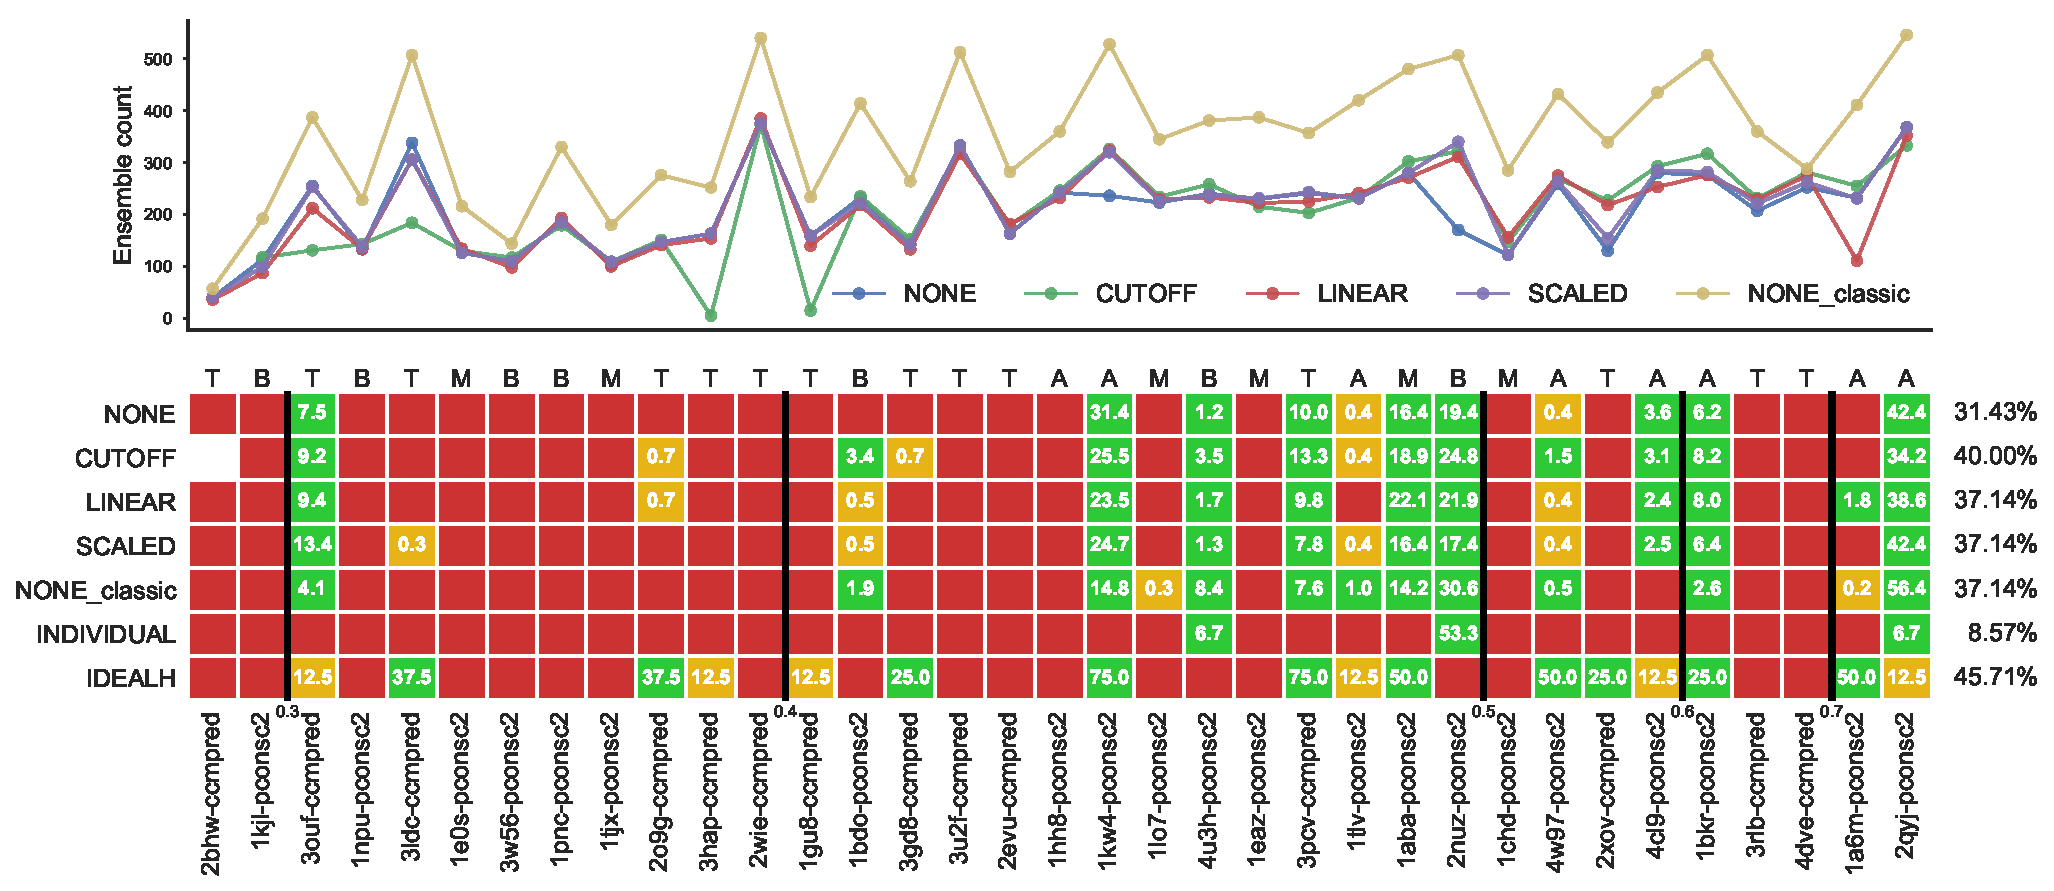
\includegraphics[width=\textwidth]{ample_decoys_mrsuccesstarget.pdf}
\caption[Molecular Replacement summary of decoy-subselected AMPLE ensembles]{Molecular Replacement summary of decoy-subselected AMPLE ensembles. AMPLE-generated ensemble counts illustrated at the top with Molecular Replacement results in grid below: red cell equates to no solution; orange to a singleton solution; and green to multiple solutions. The number in the orange and green cells indicates the percentage of ensemble search models leading to structure solutions. One letter code above each column indicates the target fold: ``T'' for transmembrane; ``A'' for all-\textalpha; ``B'' for all=\textbeta; ``M'' for mixed \textalpha-\textbeta). Percentage alongside each row indicates the number of targets with solutions by each strategy. Targets are sorted from left to right with increasing median TM-score of the starting decoy set. The black lines highlight TM-score thresholds from 0.3 to 0.7 from left to right. The subselection strategy \textit{IDEALH} refers AMPLE's ideal helix library.}
    \label{fig:ample_decoys_mrsuccesstarget}
\end{figure}

The \textit{CUTOFF} method yields the highest number of structure solutions based on AMPLE-generated ensemble search models whilst generating the fewest search models. In fact, this subselection strategy has generated no ensemble search models for target 2bhw. Furthermore, the \textit{CUTOFF} method achieves amongst the best ratio of search models leading to structure solution compared to the total number generated. 

In few exceptions, only a singleton AMPLE search model lead to a structure solution (orange cells in \cref{fig:ample_decoys_mrsuccesstarget}). Upon closer inspection, 71\% of all singleton solutions were achieved with AMPLE ensemble search models contanining at least 30\% of the target sequence. Twenty-nine percent of the singleton solutions contain at least 50\% of the target sequence, whilst none contain more than 70\%. Three out of four search models with less than 30\% of the target sequence were derived from the PCONSC2 decoy set predicted for the ketosteroid transcriptional regulator KstR2 (\gls{pdb} ID: 4w97) sequence and contained one, two or three small helical fragments.  

The rank order of targets by median TM-score of the initial starting decoy set in \cref{fig:ample_decoys_mrsuccesstarget} shows that no decoy set with median TM-score of less than 0.3 score units lead to structure solution albeit only two such cases exist in the dataset. With increasing median TM-score, i.e. increasing similarity between the decoy set and its reference target struture, the chances appear to increase to achieve structure solution. Beyond a threshold of 0.4 TM-score units, structure solutions are much more likely (over 50\% of targets solved with one of the four subselection strategies), which highlights AMPLE's success in processing such accurate decoy sets appropriately.

Finally, a comparison of decoy-derived search models and AMPLE's simplistic ideal helix library \cite{Thomas2015-wu} in \gls{mr} was done. Ideal helices achieved the most structure solutions solving nearly 46\% of all targets (\cref{fig:ample_decoys_mrsuccesstarget}). In particular, ideal helices achieved structure solutions for more transmembrane targets. Eight out of 14 transmembrane targets were solved with at least one ideal helix, which compares to six out of 14 for all decoy-based search models combined. Ideal helices also managed to near identical results for all-\textalpha\ and mixed \textalpha-\textbeta\ targets in the set compared to decoy-derived search models. However, three structure solutions for all-\textbeta\ targets are intractable.

\section{Discussion}
